\documentclass[11pt]{article}
\usepackage{fontspec}
\setmainfont{DejaVu Serif}
\usepackage{amsmath,amssymb}
\usepackage{geometry}\geometry{margin=2.3cm}
\usepackage{xcolor}\usepackage{graphicx}\usepackage{enumitem}\usepackage{booktabs}
\usepackage[hidelinks]{hyperref}
\definecolor{ink}{HTML}{16212e}\definecolor{accent}{HTML}{1f5fa8}\definecolor{soft}{HTML}{eef3fb}
\definecolor{warn}{HTML}{a8341f}\definecolor{good}{HTML}{16a34a}
\color{ink}
\newcommand{\key}[1]{\par\medskip\noindent\colorbox{soft}{\parbox{\dimexpr\linewidth-2\fboxsep}{\textcolor{accent}{\textbf{Κλειδί:}}\ #1}}\par\medskip}
\newcommand{\ex}[1]{\par\smallskip\noindent\textbf{\textcolor{accent}{Παράδειγμα.}}\ #1\par\smallskip}
\newcommand{\analogy}[1]{\par\smallskip\noindent\textit{\textbf{Αναλογία:}\ #1}\par\smallskip}
\newcommand{\warnb}[1]{\par\medskip\noindent\colorbox{soft}{\parbox{\dimexpr\linewidth-2\fboxsep}{\textcolor{warn}{\textbf{Προσοχή:}}\ #1}}\par\medskip}
\setlength{\parskip}{0.5em}\setlength{\parindent}{0pt}

\title{\textbf{Φροντιστήριο: Τα τεστ που κάνουμε σε μια στρατηγική}\\[3pt]
\large Πώς ξεχωρίζουμε το πραγματικό κέρδος από την τύχη και τα κόστη\\[-1pt]
\normalsize\textcolor{accent}{cost-survivability $\cdot$ turnover $\cdot$ no-trade band $\cdot$ durability $\cdot$ leak-free}}
\author{QUANTIQ / AGEL AI --- Stefanos Drakos}\date{\today}

\begin{document}
\maketitle\thispagestyle{empty}

\noindent Πριν βάλουμε ένα ευρώ, μια στρατηγική περνά από μια σειρά τεστ. Σκοπός τους είναι ένας:
να ξεχωρίσουν το \textbf{πραγματικό edge} από (α) την \textbf{τύχη} και (β) τα \textbf{κόστη}.
Τα περισσότερα «κερδοφόρα» συστήματα πεθαίνουν σε ένα από τα δύο. Όλα τα νούμερα εδώ είναι από τα
δικά μας πραγματικά πειράματα (paper5, δωρεάν Yahoo δεδομένα + live eToro spreads).

\tableofcontents
\bigskip

\section{Gross vs Net — μικτό vs καθαρό}
\textbf{Gross} = το κέρδος αγνοώντας τα έξοδα. \textbf{Net} = μετά τα κόστη συναλλαγών.
\analogy{Μικτός vs καθαρός μισθός. Σημασία έχει μόνο αυτό που μένει στην τσέπη.}
\key{Ένα edge που εξαφανίζεται net \emph{δεν} είναι edge. Πάντα αναφέρουμε το net.}

\section{IR (Information Ratio) — πόσο ομαλά κερδίζεις}
\[ \mathrm{IR}=\sqrt{252}\,\frac{\bar r}{\sigma_r} \]
Κέρδος ανά μονάδα ρίσκου, ετησιοποιημένο. $\bar r$ ο μέσος ημερήσιος, $\sigma_r$ η μεταβλητότητά του.
\analogy{Δύο άνθρωποι βγάζουν τα ίδια λεφτά τον χρόνο· ο ένας σταθερά, ο άλλος με τρελές ανεβοκατεβασιές.
Ο πρώτος έχει υψηλό IR.} IR $\approx 0.5$--$0.8$ = αξιοπρεπές, IR $>1$ = πολύ καλό.

\section{Turnover — πόσο συχνά μπαινοβγαίνεις}
Είναι το άθροισμα των αλλαγών θέσης. Κάθε φορά που αλλάζεις θέση πληρώνεις το \textbf{spread}.
\analogy{Κάθε μπαινοβγαίνεις στο ταξί πληρώνεις «σημαία». 100 διαδρομές = 100 σημαίες, ακόμα κι αν
η κάθε διαδρομή είναι μικρή.}
\key{Στα intraday το turnover είναι τεράστιο (\textasciitilde400/έτος vs \textasciitilde88 daily) — γι' αυτό τα κόστη
σκοτώνουν τα intraday συστήματα πρώτα.}

\section{Break-even bps — το cost-survivability τεστ}
Το κεντρικό τεστ. Ανεβάζουμε σιγά-σιγά το κόστος (σε bps, όπου $1$ bp $=0.01\%$) μέχρι το net κέρδος
να μηδενιστεί. Αυτό το σημείο = το \textbf{break-even}: πόσο ακριβό «εισιτήριο» αντέχει το edge σου.
\analogy{Πόσο ακριβό διόδιο αντέχει το ταξίδι σου πριν βγει ασύμφορο.}
\ex{Τα πραγματικά μας αποτελέσματα:}
\begin{center}\small
\begin{tabular}{lrr}
\toprule
Config & break-even & ετυμηγορία \\
\midrule
ETF intraday (4h) απλό & $\sim 0.3$ bps & \textcolor{warn}{νεκρό} \\
Crypto 4h (αργό) & $\sim 25$ bps & οριακό \\
Crypto 4h + no-trade band & $>80$ bps & \textcolor{good}{ζωντανό} \\
Crypto daily + band & $>80$ bps & \textcolor{good}{ζωντανό} \\
\bottomrule
\end{tabular}
\end{center}
\key{Συγκρίνουμε το break-even με το \emph{πραγματικό} κόστος. Live eToro crypto spreads: median
$\sim 10$ bps (3--32). Break-even $>80$ bps $\gg 10$ bps $\Rightarrow$ \textcolor{good}{επιβιώνει με μεγάλο margin}.}

\section{Αναλυτικό παράδειγμα με νούμερα (βήμα-βήμα)}
Ένα μικρό παράδειγμα 5 ημερών, 1 μετοχής, που μπορείς να ακολουθήσεις με το χέρι.

\textbf{Βήμα 1 --- το ημερήσιο κέρδος.} Κάθε μέρα κρατάς θέση $w$ ($+1$ long, $-1$ short)· η μετοχή
κινείται κατά $r\%$ την επόμενη μέρα· \textbf{κέρδος της μέρας $= w\times r$}.
\begin{center}\small
\begin{tabular}{ccccc}
\toprule
Μέρα & θέση $w$ & κίνηση $r$ & κέρδος $w\times r$ & turnover $|w_t-w_{t-1}|$ \\
\midrule
1 & $+1.0$ & $+2.0\%$ & $+2.0\%$ & $1.0$ \\
2 & $+1.0$ & $-1.0\%$ & $-1.0\%$ & $0$ \\
3 & $-1.0$ & $-2.0\%$ & $+2.0\%$ & $2.0$ \\
4 & $+1.0$ & $+1.0\%$ & $+1.0\%$ & $2.0$ \\
5 & $+1.0$ & $+0.5\%$ & $+0.5\%$ & $0$ \\
\bottomrule
\end{tabular}
\end{center}
Ροή gross κέρδους: $[+2.0,\,-1.0,\,+2.0,\,+1.0,\,+0.5]\%$. Μέσο turnover $=5.0/5=1.0$/μέρα.

\noindent\textbf{Προσοχή στο turnover --- γιατί η Μέρα 3 είναι $2$ και όχι $1$:} το turnover
$=|w_t-w_{t-1}|$ μετράει τον \emph{όγκο που εμπορεύτηκες}. Η Μέρα 3 πάει $+1.0\to-1.0$, δηλαδή
$|-1-(+1)|=2$, γιατί κάνεις \emph{δύο} πράξεις: (1) \textbf{κλείνεις} το $+1$ long και (2)
\textbf{ανοίγεις} το $-1$ short --- πληρώνεις spread \emph{δύο} φορές. Αντίθετα, Μέρα 2 ($+1\to+1$)
$=0$ (απλώς κρατάς, \textbf{δωρεάν})· Μέρα 1 ($0\to+1$) $=1$ (μόνο ανοίγεις).
\analogy{Το να \textbf{γυρίζεις κατεύθυνση} (long$\leftrightarrow$short) κοστίζει \emph{διπλά}· το να
\textbf{κρατάς} είναι δωρεάν. Γι' αυτό τα νευρικά σήματα (πολλά flips) συσσωρεύουν τεράστιο turnover,
και γι' αυτό το no-trade band / αργό σήμα --- που μειώνουν τα flips --- ανεβάζουν το break-even.}

\textbf{Βήμα 2 --- το IR.}
\begin{enumerate}[leftmargin=1.5em,nosep]
\item Μέσος $=\frac{2.0-1.0+2.0+1.0+0.5}{5}=\mathbf{0.90\%}$/μέρα.
\item Αποκλίσεις από τον μέσο $[+1.1,-1.9,+1.1,+0.1,-0.4]$· τετράγωνα αθροίζουν $6.20$· $/5=1.24$·
$\sqrt{\,}=\mathbf{1.11\%}$ (τυπική απόκλιση).
\item Ημερήσιο IR $=0.90/1.11=\mathbf{0.81}$· ετήσιο $=0.81\times\sqrt{252}$.
\end{enumerate}
Το $\div$ τυπική απόκλιση = «κέρδος ανά ρίσκο»: ίδιος μέσος αλλά πιο νευρική ροή → χαμηλότερο IR.

\textbf{Βήμα 3 --- ανεβάζουμε τα bps.} Κόστος $=\frac{s}{10000}\times$turnover. Το κλειδί είναι μια ευθεία:
\[ \text{μέσο net} = \text{μέσο gross} - (\text{turnover}\times s). \]
\begin{center}\small
\begin{tabular}{cccc}
\toprule
$s$ (bps) & κόστος/μέρα $=1.0\times s$ & μέσο net/μέρα & \\
\midrule
$0$ & $0$ & $0.90\%$ & \\
$10$ & $0.10\%$ & $0.80\%$ & \\
$50$ & $0.50\%$ & $0.40\%$ & \\
$\mathbf{90}$ & $\mathbf{0.90\%}$ & $\mathbf{0.00\%}$ & $\leftarrow$ break-even \\
$120$ & $1.20\%$ & $-0.30\%$ & (χάνεις) \\
\bottomrule
\end{tabular}
\end{center}
\textbf{Βήμα 4 --- break-even} = όπου το net μηδενίζεται:
\[ s^\star=\frac{\text{μέσο gross}}{\text{turnover}}=\frac{0.90\%}{1.0}=0.90\%=\mathbf{90\ \text{bps}}. \]
\key{Από τον τύπο $s^\star=\text{gross}/\text{turnover}$ εξηγούνται τα πάντα: \emph{intraday πεθαίνει} (turnover
$30$ αντί $1$ $\Rightarrow$ $s^\star=3$ bps), το \emph{no-trade band σώζει} (κόβει turnover $\Rightarrow$
ανεβάζει $s^\star$), το \emph{crypto βοηθάει} (μεγαλύτερο gross $\Rightarrow$ μεγαλύτερο $s^\star$).}

\section{No-trade band — μη αλλάζεις λωρίδα για ένα εκατοστό}
Αλλάζεις θέση μόνο αν ο στόχος κινηθεί \emph{αρκετά}· αγνοείς τα μικρο-wiggles (που είναι κυρίως
θόρυβος). \analogy{Δεν στρίβεις το τιμόνι για κάθε μικρή ανωμαλία του δρόμου — μόνο για πραγματικές
στροφές.}
\key{Έκοψε turnover \textbf{$\times 35$} ($0.07\to0.002$) και ανέβασε το break-even από $5$ σε $>80$ bps.
Ο πιο ισχυρός μοχλός που έχουμε — και «καθάρισε» τη στρατηγική.}

\section{Vol-targeting — γκάζι ανάλογα με τον δρόμο}
Κρατάμε σταθερό το ρίσκο: μικραίνουμε τη θέση όταν η αγορά είναι ταραγμένη (υψηλή μεταβλητότητα),
μεγαλώνουμε όταν είναι ήρεμη. Ελέγχει το drawdown και είναι «ο διακόπτης ρίσκου/κέρδους».

\section{Durability by year — αθλητής κάθε σεζόν, όχι μια καλή χρονιά}
Σπάμε το κέρδος \textbf{ανά έτος}. Το κρίσιμο: δουλεύει και σε \emph{bear} χρονιά, ή μόνο σε bull;
\analogy{Ένας παίκτης που σκοράρει κάθε σεζόν είναι αληθινός· ένας με μία καλή χρονιά ήταν τυχερός.}
\ex{Crypto banded daily, net IR ανά έτος (το $2022$ ήταν crypto crash, BTC $-65\%$):}
\begin{center}\small
\texttt{2020:+2.3\quad 2021:+1.4\quad \textbf{2022:+1.2}\quad 2023:+0.7\quad 2024:+1.2\quad 2026:+2.9}
\end{center}
Κέρδος \textbf{μέσα στο crash} (το trend-following έκανε de-risk/short) $\Rightarrow$ \textcolor{good}{αληθινό
σήμα, όχι bull-artifact}. Συνολικά: net IR $1.27$, $t_{\mathrm{NW}}=2.74$, maxDD μόλις $-8\%$.

\section{Διαβάζοντας μια πραγματική καμπύλη κεφαλαίου}
Όλα τα νούμερα προκύπτουν από \emph{μία} σειρά: τις καθημερινές καθαρές αποδόσεις $net$. Η εικόνα
δείχνει το crypto banded-daily (το config με net IR $1.27$): πάνω το κεφάλαιο, κάτω το drawdown.

\begin{center}
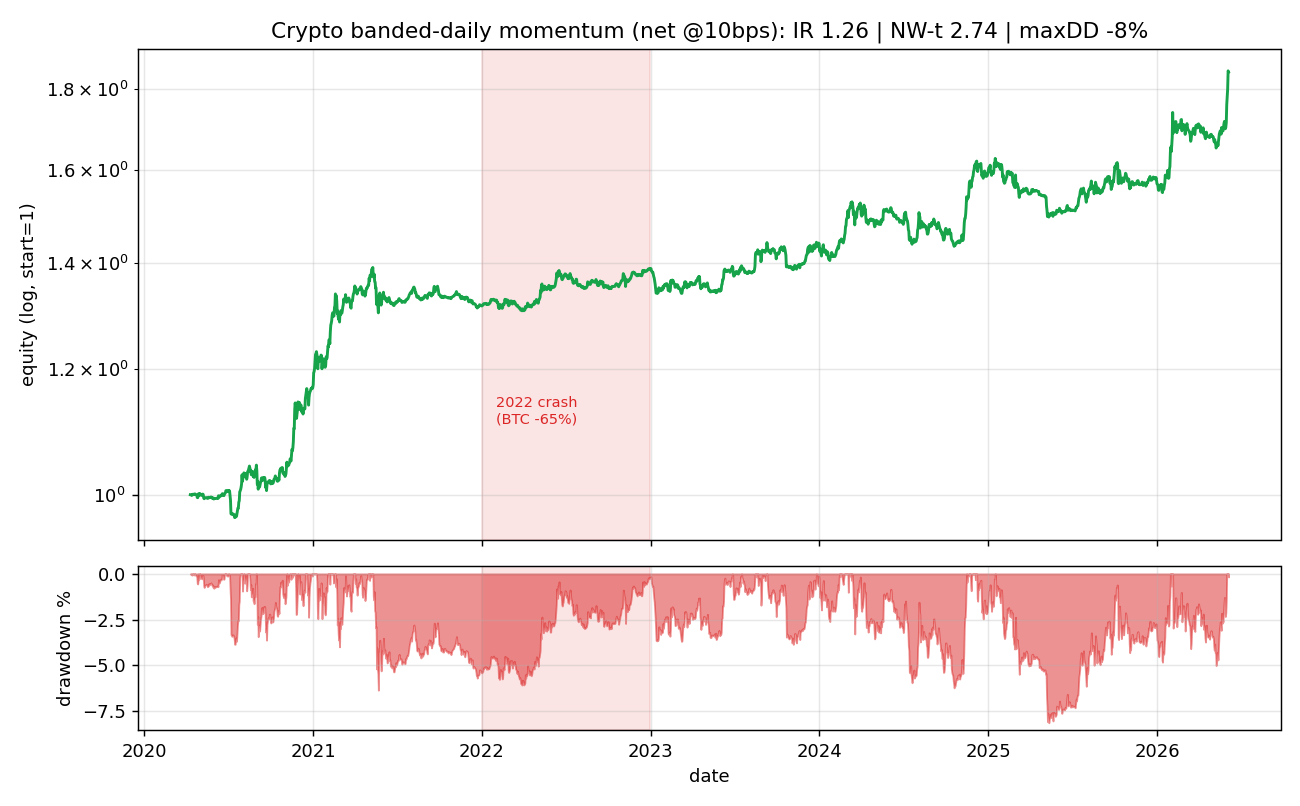
\includegraphics[width=0.93\textwidth]{figures/fig_crypto_pnl.png}
\end{center}

Πώς διαβάζεται και πώς βγαίνει κάθε νούμερο:
\begin{itemize}[leftmargin=1.4em]
\item \textbf{Πράσινη καμπύλη = κεφάλαιο.} Ξεκινάς με $1$· κάθε μέρα πολλαπλασιάζεις $\times(1+net)$.
Συνολικά $+84\%$ σε $\sim 6$ χρόνια (log κλίμακα, ώστε οι ποσοστιαίες αλλαγές να φαίνονται σταθερές).
\item \textbf{IR $=1.26$} $=$ πόσο \emph{ομαλά} ανεβαίνει: μέσος ημερήσιος $\div$ τρέμουλο, $\times\sqrt{365}$.
Ευθεία ανηφόρα $\to$ υψηλό IR· πριονωτή $\to$ χαμηλό.
\item \textbf{maxDD $=-8\%$} (κόκκινο, κάτω) $=$ η χειρότερη πτώση από κορυφή σε πάτο της πράσινης
καμπύλης. Για σύγκριση, το buy-and-hold crypto έχει maxDD $\sim-70\%$ — το trend-following το απέφυγε.
\item \textbf{NW-t $=2.74$} $=$ πόσο σίγουροι ότι η άνοδος δεν είναι τύχη (μέσος $\div$ τυπικό σφάλμα,
διορθωμένο για autocorrelation)· $>2$ σημαίνει $\sim 99\%$ σιγουριά.
\item \textbf{Η σκιασμένη ζώνη $2022$} (BTC $-65\%$): η καμπύλη \emph{δεν} βυθίζεται — το trend ήταν κάτω,
οπότε η θέση έγινε short/μηδέν και η στρατηγική \textbf{κέρδισε μέσα στο crash}. Αυτό είναι το «αληθινό
σήμα, όχι bull-artifact»: το drawdown panel μένει ρηχό ακριβώς εκεί που το buy-and-hold κατέρρευσε.
\end{itemize}
\key{Το μάτι ψάχνει τρία πράγματα σε μια καμπύλη: \emph{σταθερή} ανηφόρα (υψηλό IR), \emph{ρηχά}
drawdowns (καλό maxDD), και ότι \emph{κρατάει στα bear} (durability). Και τα τρία είναι εδώ.}

\section{Leak-free \& Out-of-sample — εξετάσεις χωρίς τις απαντήσεις}
Δεν χρησιμοποιούμε ποτέ μελλοντική πληροφορία: η μεταβλητότητα και το σήμα υπολογίζονται \emph{μόνο
από το παρελθόν}, και η είσοδος γίνεται την \emph{επόμενη} μπάρα ($T{+}1$). Τεστάρουμε σε δεδομένα που
το μοντέλο \emph{δεν είδε}. \analogy{Διαγώνισμα σε ύλη που δεν είχες δει τις λύσεις — αλλιώς ο βαθμός
είναι ψεύτικος.}
\warnb{Το πιο συχνό «κρυφό λάθος»: να βάλεις μελλοντική πληροφορία (π.χ. vol όλης της περιόδου) — δίνει
εντυπωσιακά backtest που πεθαίνουν live.}

\section{Η αλυσίδα (η σειρά που ρωτάμε)}
\begin{enumerate}[leftmargin=1.5em]
\item \textbf{Υπάρχει edge;} → gross IR.
\item \textbf{Επιβιώνει στα κόστη;} → turnover + break-even vs πραγματικό spread.
\item \textbf{Σε κάθε regime;} → durability by year (το $2022$ τεστ).
\item \textbf{Είναι αληθινό, όχι τύχη;} → Newey-West $t>2$, Deflated Sharpe.
\end{enumerate}
Μόνο αν περάσει \emph{και τα τέσσερα}, αξίζει να χτιστεί/τραδαριστεί. Στο paper5 ο νικητής μέχρι τώρα:
\textbf{crypto momentum με no-trade band + vol-target}, που πέρασε και τα τέσσερα (incl. το $2022$).

\vfill
\noindent\rule{\linewidth}{0.4pt}\\[2pt]
\footnotesize Νούμερα: paper5 cost-survivability \& regime-stress (Yahoo, 2013--2026· crypto 2020--2026),
live eToro crypto spreads (2026). Όλα net-of-cost, leak-free, out-of-sample.
\end{document}
